% This is what ChatGPT came up with for Figure 1 in the Metcalfe + Boggs Paper

% A rough approximation of "Fig. 1. A two-segment Ethernet."
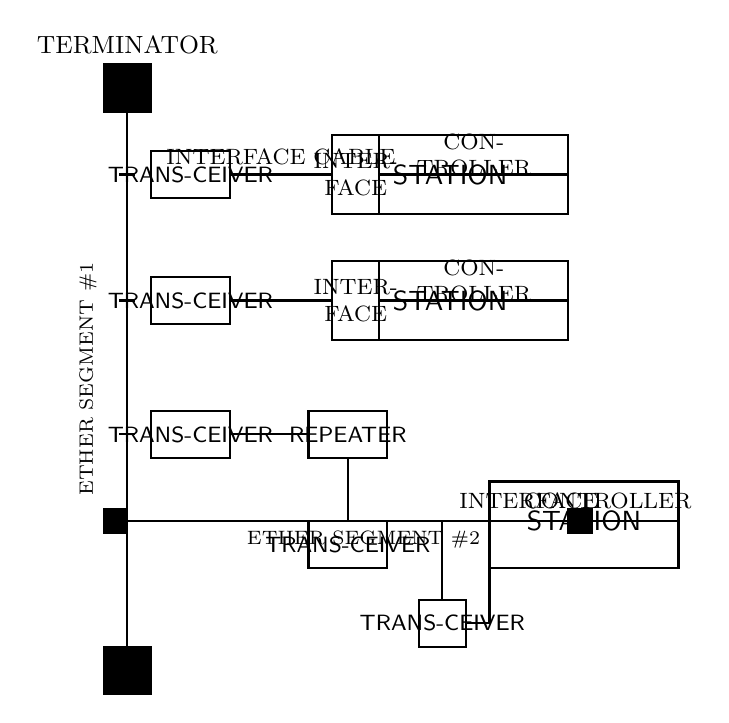
\begin{tikzpicture}[font=\sffamily, line width=0.8pt]
    %----------------------
    % ETHER SEGMENT #1 (vertical)
    %----------------------
    % Draw top terminator
    \filldraw[black] (-0.3,8) rectangle (0.3,7.4);
    \node[above, font=\small] at (0,8) {TERMINATOR};

    % Draw vertical cable
    \draw (0,7.4) -- (0,0.6);

    % Label the vertical cable
    \node[rotate=90, font=\scriptsize] at (-0.5,4) {ETHER SEGMENT \#1};

    % Draw bottom terminator on segment #1
    \filldraw[black] (-0.3,0.6) rectangle (0.3,0.0);

    %----------------------
    % FIRST TRANSCEIVER + STATION
    %----------------------
    % The transceiver "tap" at around y=6.6
    \draw[thick] (-0.1,6.6) -- (0.1,6.6);
    \draw[rectangle, fill=white] (0.3,6.9) rectangle (1.3,6.3);
    \node at (0.8,6.6) {\footnotesize TRANS-\\CEIVER};

    % Cable to station (interface,controller,station)
    \draw (1.3,6.6) -- (2.6,6.6);
    \node[above, font=\footnotesize] at (1.95,6.6) {INTERFACE CABLE};

    % Station block (Interface, Controller, Station)
    % We'll stack small rectangles
    % Outer "station" box at (2.6,6.6) + 4 cm width
    \draw (2.6,7.1) rectangle (5.6,6.1);  % large station box
    \node at (4.1,6.6) {STATION};
    % Put a narrow interface/controller label block on left
    \draw (2.6,7.1) -- (3.2,7.1) -- (3.2,6.1) -- (2.6,6.1) -- cycle;
    % Sub-boxes for interface, controller
    \node[align=center, font=\footnotesize] at (2.9,6.6) {INTER-\\FACE};
    \draw (3.2,7.1) -- (3.2,6.1);

    \draw (3.2,6.6) -- (5.6,6.6);

    \node[align=center, font=\footnotesize] at (4.4,6.85) {CON-\\TROLLER};

    %----------------------
    % SECOND TRANSCEIVER + STATION
    %----------------------
    % Another tap at y=5.0
    \draw[thick] (-0.1,5.0) -- (0.1,5.0);
    \draw (0.3,5.3) rectangle (1.3,4.7);
    \node at (0.8,5.0) {\footnotesize TRANS-\\CEIVER};

    % Cable to second station
    \draw (1.3,5.0) -- (2.6,5.0);

    % Second station block
    \draw (2.6,5.5) rectangle (5.6,4.5);
    \node at (4.1,5.0) {STATION};
    % Left label region
    \draw (2.6,5.5) -- (3.2,5.5) -- (3.2,4.5) -- (2.6,4.5) -- cycle;
    \node[font=\footnotesize, align=center] at (2.9,5.0) {INTER-\\FACE};
    \draw (3.2,5.0) -- (5.6,5.0);
    \node[font=\footnotesize, align=center] at (4.4,5.25) {CON-\\TROLLER};

    %----------------------
    % REPEATER + bridging to ETHER SEGMENT #2 (horizontal)
    %----------------------
    % Tap at y=3.3 for the transceiver
    \draw[thick] (-0.1,3.3) -- (0.1,3.3);
    \draw (0.3,3.6) rectangle (1.3,3.0);
    \node at (0.8,3.3) {\footnotesize TRANS-\\CEIVER};

    % Repeater to transceiver below it
    \draw (1.3,3.3) -- (2.3,3.3);
    \draw (2.3,3.6) rectangle (3.3,3.0);
    \node at (2.8,3.3) {\footnotesize REPEATER};

    \draw (2.8,3.0) -- (2.8,2.2);
    \draw (2.3,2.2) rectangle (3.3,1.6);
    \node at (2.8,1.9) {\footnotesize TRANS-\\CEIVER};

    % Horizontal Ether Segment #2
    \draw (0,2.2) -- (5.6,2.2); % connect from vertical cable to the next cable
    % A black square 'junction'
    \filldraw[black] (-0.3,2.35) rectangle (0,2.05);

    % Label horizontal cable
    \node[below, font=\scriptsize] at (3,2.2) {ETHER SEGMENT \#2};

    % Terminator on the far right
    \filldraw[black] (5.6,2.35) rectangle (5.9,2.05);

    %----------------------
    % Station on ETHER SEGMENT #2
    %----------------------
    % A transceiver connected to the station
    \draw[thick] (4,2.2) -- (4,1.2);
    \draw (3.7,1.2) rectangle (4.3,0.6);
    \node at (4,0.9) {\footnotesize TRANS-\\CEIVER};

    % Station block above
    \draw (4.6,2.7) rectangle (7.0,1.6); 
    \node at (5.8,2.2) {STATION};
    % interface, controller boxes stacked
    \draw (4.6,2.2) -- (7.0,2.2);
    \draw (4.6,1.6) -- (7.0,1.6);
    \node[font=\footnotesize] at (5.1,2.45) {INTERFACE};
    \node[font=\footnotesize] at (6.1,2.45) {CONTROLLER};

    % Cable from transceiver into the station
    \draw (4.3,0.9) -- (4.6,0.9) -- (4.6,1.6);

\end{tikzpicture}

